% - question answering framework is suited to give generalized questions as input and even then expect the model to learn correct answer spans

% - QA effectiveness on identifying accurate entity boundaries (which is key for NER) is already proven by its recent success in NER

% - QA model is found to give high precision/recall for even very generalized entity types (like Genes). This motivates us to gneralize and try bringing all extractable entities under one bucket (motivation for span detection)

% The BERT model is trained on a vast English corpus and the deeply interconnected transformer architecture ensures that the so-called foundational model learns some generalized semantics and language attributes which can be fine-tuned and reoriented to suit for a variety of NLP tasks, one such being NER.

% In the NLP domain, there are several standardized problem settings or paradigms, like sequence labeling, sentence classification. An NLP application can be approached (or solved) through several of these problem settings. For example, one way of looking at NER task is through sequence labeling where each token of a sequence is to be labeled into an output class, like \texttt{Person}, \texttt{Organization}. The NER task has been traditionally looked at from this perspective. However, recently the question-answering setting has gained popularity for NER, where a question is fed as plain text, like, "Where is the Person mentioned in the text?" along with the sentence input and a model is trained to output the right span where the entity in question is present. \cite{} show the effectiveness of the question-answering paradigm for NER over the BERT architecture. Here on, we refer to this as the \texttt{BERT-QA} setup. We implemented the \texttt{BERT-QA} setup, trained it on multiple datasets (OntoNotes, BioNLP13CG, WNUT) and qualitatively studied the model outputs to draw two broad findings:

% \begin{enumerate}
%     \item \textbf{Finding 1}: Entity mentions belonging to the same entity type can occur in different parts of the sentence depending on sentence style.
    
%     \item \textbf{Finding 2}: Entity mentions belonging to different entity types can occur in similar parts of the sentence.
% \end{enumerate}

% The findings are substantiated through examples in Table \ref{tab:ner_problem_ex}. Based on the findings, we can conclude that identifying entity mentions and inferring their entity types can be decoupled and treated as separate tasks. This gives the advantage that entity mention extraction rules can be shared across entity types and in case of datasets with high class imbalance, the rare entities can benefit from rules derived from mentions of the frequent ones. 

% This motivates us to break down the NER task into two sub-tasks, \textit{Span Detection} and \textit{Span Classification}, each of which are trained independent of each other. \textit{Span Detection} is entity-type agnostic and forms generalized rules to identify mention spans. The \textit{Span Classification} stage takes these mention span outputs from the previous stage and associates them with their entity types.

% In fact, through the similarity of our results as shown later in the paper, an NER system performing well on a dataset which does not violate the findings stated above, inherently is performing the span detection and classification tasks separately. 

As the name suggests, \modelname{} performs NER through a combination of two independently trained modules  -- \spandetect{} and \spanclass{}, both of which are modeled as question-answering tasks. Both modules use BERT-base as the underlying architecture. \spandetect{} identifies all required mention spans in a given sentence irrespective of entity type by learning entity-agnostic extraction rules. This helps rare entity types borrow knowledge from the more common ones. These extracted mention spans are fed one-by-one to \spanclass{} which reanalyses them in the sentence structure and classifies them into an entity type. In this way, both modules, even though being separate from each other, have complete access to full sentence structure and do not suffer from lack of any essential information that may be required for their sub-tasks. Both modules can be trained independently, in parallel. Even if done sequentially, these sub-tasks are much simpler to learn than the overall NER task and this gives \modelname{} a significant efficiency boost and better performance than corresponding baselines which train a single NER model. Figure~\ref{fig:framework} illustrates how \modelname{} works. 

% Our method is completely different from other span classification-based methods~\cite{li2020MRC,Jiang20,Ouchi20}, which consider all possible spans up a predetermined length in a input sequence. 

\begin{figure*}[h!]
    \centering
    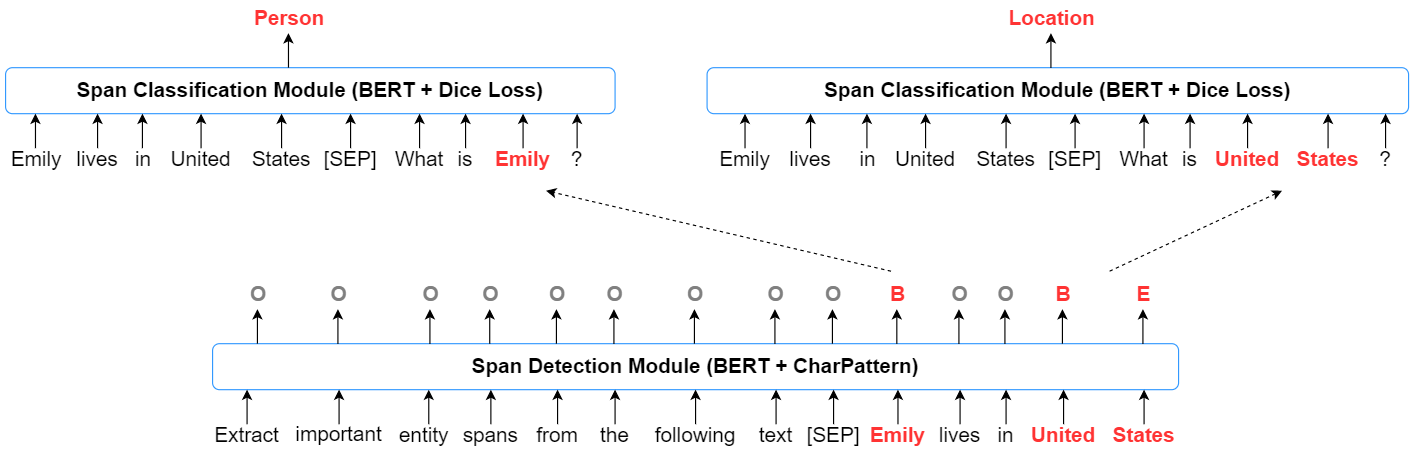
\includegraphics[width=0.9\linewidth]{framework6.png}
    \caption{Overview of \modelname. Sentence \textit{``Emily lives in United States"} is fed as input to \spandetect{} which identifies two mention spans. Each span is then queried with \spanclass{} which assigns them the most probable entity type. \texttt{CharPattern} refers to character and pattern features described in the \textit{Span Detection} section.}
    \label{fig:framework}
\end{figure*}